%Related Studies
\section{Related Studies}

Estimating ensemble width represents a unique approach within binaural audio literature, which more commonly focuses on identifying the locations of individual sound sources \cite{benaroya_binaural_2018,ma_speech_2016,ma_exploiting_2017,may_probabilistic_2011,may_robust_2015}. While analyzing individual sound sources might seem more useful because it yields more precise information, such methods have limitations that hinder their practical application. These include a limited or predetermined number of sound sources and a predetermined type of audio signal—typically speech \cite{benaroya_binaural_2018,ma_speech_2016,may_probabilistic_2011,may_robust_2015,yang_deepear_2024}. The ensemble approach serves as a workaround for these limitations by providing useful spatial information without such constraints.

Traditional audio localization methods often rely on arrays with more than two microphones to improve precision through additional channel information \cite{pavlidi_real-time_2012,hahmann_sound_2022,liu_sound_2022}. While adding microphones can enhance precision through additional channel information, they do not utilize binaural hearing principles, rendering them ineffective for binaural recording assessment. By contrast, as Yang et al. demonstrate, systems using only two microphones can achieve superior localization accuracy by integrating binaural cues \cite{yang_deepear_2024}.

The majority of studies on sound source localization in binaural recordings concentrate on the localization of individual sources in isolation, typically referred to as Direction of Arrival (DoA) \cite{benaroya_binaural_2018,ma_speech_2016,ma_exploiting_2017,may_probabilistic_2011,may_robust_2015}. Although this granular approach provides detailed information, the existing methods require \textit{a~priori} knowledge of the number of sources, usually limiting analysis to between one and six sources. These constraints present significant challenges in real-life scenarios, where such advance knowledge is unavailable. Moreover, these methods have been developed primarily for homogeneous signals, especially speech, making them impractical for real-world binaural recordings where signals are often heterogeneous.

In a series of recent studies, Arthi and Sreenivas \cite{arthi_binaural_2022}, Antoniuk at al. \cite{antoniuk_blind_2023,antoniuk_ensemble_2024,antoniuk_estimating_2024}, introduced an alternative approach, treating sound sources as ensembles that can be characterized by their location and width, as illustrated in Figure \ref{fig:figx}. This method overcomes the limitations of traditional DoA approaches by focusing on ensemble characteristics rather than precise individual source locations. The approach eliminates the need for \textit{a prior} knowledge of the number of sources and has been validated across diverse musical content, including both instrumental and vocal recordings \cite{antoniuk_blind_2023,antoniuk_ensemble_2024,antoniuk_estimating_2024}.

\begin{figure}[htbp]
	\begin{center}
		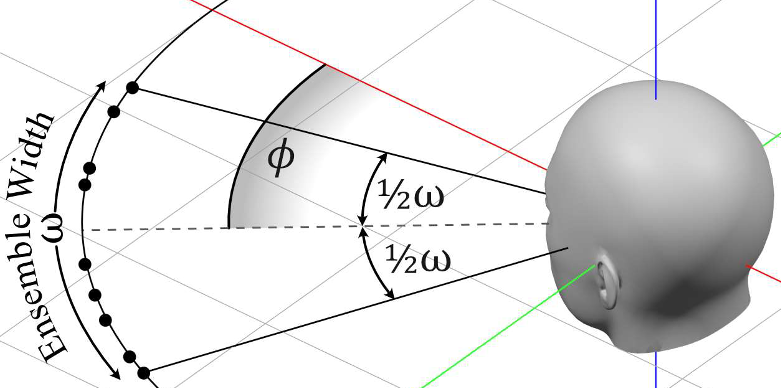
\includegraphics[width=1.0\linewidth]{img/figx.png} 
	\end{center}
	\caption{An ensemble example comprising nine point-like sound sources shown as dots. The ensemble's width is denoted by $\omega$, while $\phi$ indicates the counterclockwise position of the ensemble's center.} \label{fig:figx}
\end{figure}

This approach aligns with the second level of Rumsey's spatial audio scene-based framework \cite{rumsey_spatial_2002}, which defines three distinct levels: (1) single source, (2) scene, and (3) environment. Scene-level analysis, as described by Rumsey, better matches the human auditory system's natural source-grouping mechanisms. The approach mirrors real-world musical performance configurations where instruments and vocals occupy adjacent spatial positions. Notably, the methods incorporated in this study specifically measure physical ensemble width rather than apparent ensemble width---two related but distinct parameters whose relationship warrants further investigation.
